
\chapter{Implementace}
\label{chap:Imp}

\pagestyle{plain}
  
    \section{Datov\'{e} struktury pro implementaci LBM}
    \label{sec:MPI}

        V t\'{e}to sekci se zam\v{e}\v{r}\'{\i}me na popis datov\'{y}ch struktur, kter\'{e} jsou pou\v{z}ity p\v{r}i implementaci m\v{r}\'{\i}\v{z}kov\'{e} Boltzmannovy metody. 

        Jak bylo pops\'{a}no podrobn\v{e} v t\'{e}to kapitole, podstatou LBM jsou distribu\v{c}n\'{\i} funkce, kter\'{e} jsou rozm\'{\i}st\v{e}ny na ekvidistantn\'{\i} m\v{r}\'{\i}\v{z}ce. Rozm\v{e}ry m\v{r}\'{\i}\v{z}ky jsou v p\v{r}\'{\i}pad\v{e} 3D sch\'{e}mat $N_x$, $N_y$, $N_z$. Pro ka\v{z}d\'{y} uzel m\v{r}\'{\i}\v{z}ky m\'{a}me v pam\v{e}ti ulo\v{z}enou celou sadu distribu\v{c}n\'{\i}ch funkc\'{\i}, tj. pro NSR sch\'{e}ma vyu\v{z}\'{\i}vaj\'{\i}c\'{\i} modelu $D3Q27$ to je celkem $27 N_x N_y N_z$ hodnot, pro ADR sch\'{e}ma s modelem $D3Q7$ pak jen $7 N_x N_y N_z$ hodnot.
        Nav\'{\i}c je tento algoritmus navr\v{z}en tak, aby m\v{e}l k dispozici 2 sady distribu\v{c}n\'{\i}ch funkc\'{\i}, kter\'{e} se p\v{r}i ka\v{z}d\'{e}m \v{c}asov\'{e}m kroku st\v{r}\'{\i}daj\'{\i}, tud\'{\i}\v{z} jen k ulo\v{z}en\'{\i} distribu\v{c}n\'{\i}ch funkc\'{\i} je pot\v{r}eba n\v{e}kolik pol\'{\i} o celkov\'{e} d\'{e}lce $68 N_x N_y N_z$. P\v{r}i po\v{c}\'{\i}t\'{a}n\'{\i} na grafick\'{y}ch kart\'{a}ch se tato pole se duplikuj\'{\i} mezi syst\'{e}movou pam\v{e}t\'{\i} a grafickou kartou. B\v{e}hem inicializace se pak pole kop\'{\i}ruj\'{\i} z RAM do GPU, p\v{r}i v\'{y}stupu na disk kop\'{\i}rov\'{a}n\'{\i} prob\'{\i}h\'{a} z GPU do RAM.

        D\'{a}le je zapot\v{r}eb\'{\i} definovat pole o velikosti $N_x N_y N_z$, ve kter\'{e}m budou ulo\v{z}eny hodnoty okrajov\'{y}ch podm\'{\i}nek v dan\'{e}m uzlu. Tato pole budou pot\v{r}eba dv\v{e} -- jedno pro NSR a druh\'{e} pro ADR sch\'{e}ma.

        Nakonec pak dost\'{a}v\'{a}me vzorec pro odhad celkov\'{e} pam\v{e}ti pot\v{r}ebn\'{e} pro jednu simulaci:
        
        \begin{equation}
            \mathrm{Me} = 8 \cdot 68 N_x N_y N_z + 8 \cdot V N_x N_y N_z + 2 \cdot 2 N_x N_y N_z,
        \end{equation}
        kde $\mathrm{Me} \ [\mathrm{B}]$ zna\v{c}\'{\i} celkov\'{y} odhad pot\v{r}ebn\'{e} pam\v{e}ti. Prvn\'{\i} s\v{c}\'{\i}tanec zastupuje velikost pol\'{\i} pro distribu\v{c}n\'{\i} funkce, druh\'{y} odhaduje velikost ukl\'{a}dan\'{y}ch makroskopick\'{y}ch veli\v{c}in $V \ [-]$ a t\v{r}et\'{\i} \v{c}len aproximuje pole s okrajov\'{y}mi podm\'{\i}nkami. Prvn\'{\i} dva \v{c}leny jsou typu \texttt{\lstinline{double}} s velikost\'{\i} 8 bajt\r{u}, posledn\'{\i} pak m\r{u}\v{z}e b\'{y}t ukl\'{a}d\'{a}n pouze jako \texttt{\lstinline{short int}}, tedy s velikost\'{\i} 2 bajty. Co se po\v{c}tu makroskopick\'{y}ch veli\v{c}in $V$ t\'{y}\v{c}e, jejich po\v{c}et je pro simulace v t\'{e}to pr\'{a}ci roven $5$ - slo\v{z}ky rychlosti $u_i$ pro $i \in \{1,2,3\}$, hustota $\rho$ a teplota $T$.

        \subsection{Pole pro difuzn\'{\i} koeficient}
            
            Sch\'{e}ma \v{r}e\v{s}\'{\i}c\'{\i} ADR bylo v r\'{a}mci t\'{e}to pr\'{a}ce roz\v{s}\'{\i}\v{r}eno o pole pro difuzn\'{\i} koeficient, d\'{\i}ky \v{c}emu\v{z} je mo\v{z}nost nastavit v oblasti r\r{u}znou fyzik\'{a}ln\'{\i} difuzi. Toto pole inicializujeme na po\v{c}\'{a}tku algoritmu hodnotami difuze ve v\v{s}ech bodech m\v{r}\'{\i}\v{z}ky a n\'{a}sledn\v{e} je toto pole zkop\'{\i}rov\'{a}no na grafickou kartu, kde hodnoty z n\v{e}j jsou pak pou\v{z}\'{\i}v\'{a}ny v dal\v{s}\'{\i}ch \v{c}\'{a}stech algoritmu. 

            Nap\v{r}\'{\i}klad chceme-li simulovat t\v{e}leso, kter\'{e} m\'{a} jin\'{y} difuzn\'{\i} koeficient ne\v{z} okoln\'{i} tekutina, sta\v{c}\'{\i} pro uzly n\'{a}le\v{z}\'{\i}c\'{\i} tomuto t\v{e}lesu nastavit difuzi na po\v{z}adovanou hodnotu.

        \subsection{Pozn\'{a}mky k po\v{c}\'{\i}t\'{a}n\'{\i} na v\'{\i}ce grafick\'{y}ch kart\'{a}ch}

            P\v{r}i paraleln\'{\i}m po\v{c}\'{\i}t\'{a}n\'{\i} na v\'{\i}ce grafick\'{y}ch kart\'{a}ch je cel\'{a} m\v{r}\'{\i}\v{z}ka rozd\v{e}lena do blok\r{u} dle po\v{c}tu pou\v{z}it\'{y}ch grafick\'{y}ch karet. Toto rozd\v{e}len\'{\i} v pou\v{z}it\'{e}m k\'{o}du prob\'{\i}h\'{a} v\'{y}hradn\v{e} pod\'{e}l osy $x$, viz obr\'{a}zek \ref{fig:blocks}.
            
            Pro zaji\v{s}t\v{e}n\'{\i} spr\'{a}vn\'{e} komunikace mezi jednotliv\'{y}mi bloky mezi sebou je nutn\'{e} zav\'{e}st tzv. p\v{r}ekryvy jednotliv\'{y}ch blok\r{u}. Pro ka\v{z}d\'{y} blok na ka\v{z}d\'{e} kart\v{e} alokujeme pole o 1 v\v{e}t\v{s}\'{\i} v ka\v{z}d\'{e}m sm\v{e}ru osy $x$. B\v{e}hem komunikace si soused\'{\i}c\'{\i} bloky p\v{r}ed\'{a}vaj\'{\i} informace z t\v{e}chto p\v{r}ekryv\r{u} a mohou tedy z\'{\i}skat pot\v{r}ebn\'{e} distribu\v{c}n\'{\i} funkce ze sm\v{e}r\r{u}, kter\'{e} by jinak byly nedostupn\'{e}.

            \begin{figure}[H]
                \centering
                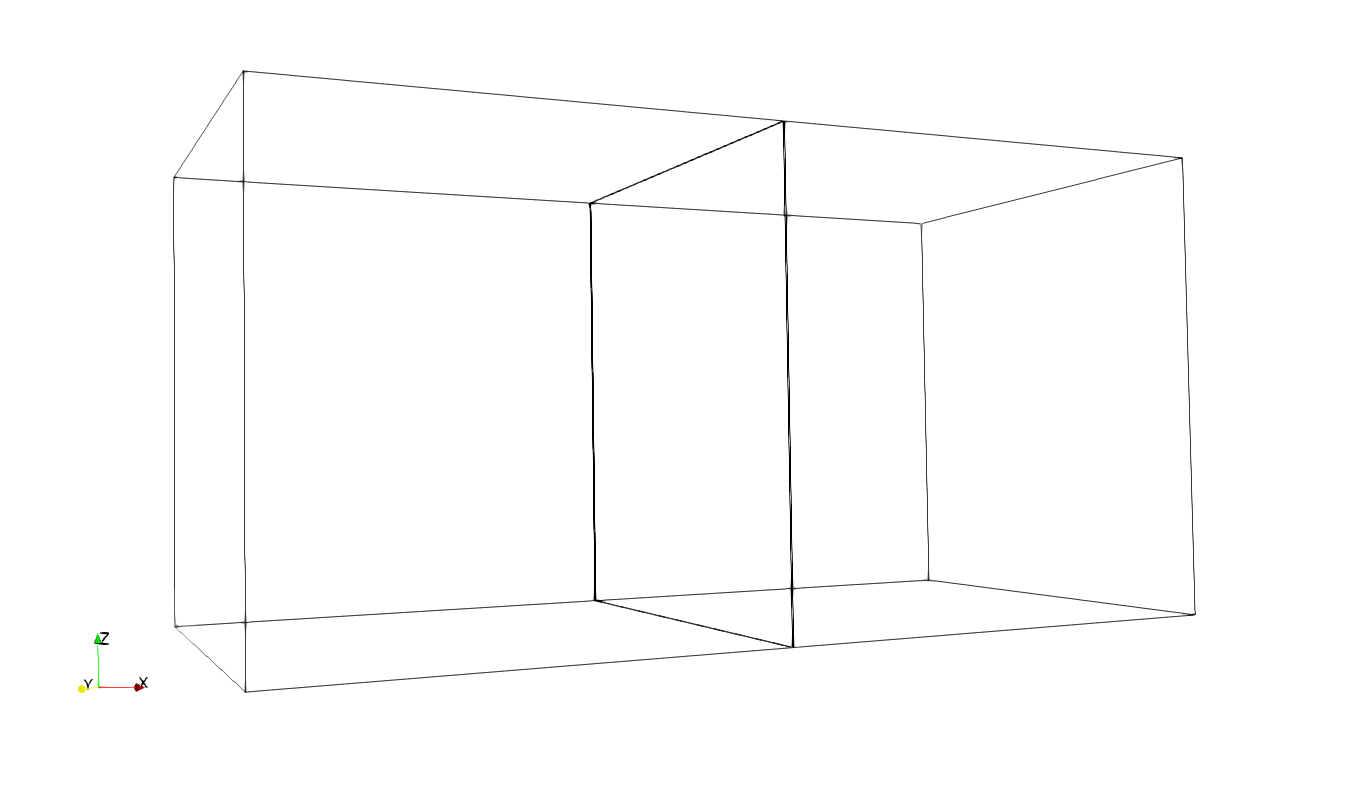
\includegraphics[width=.7\linewidth]{Img/Kapitola 2/More_GPUs_domain.png}
                \caption{Rozd\v{e}len\'{\i} v\'{y}po\v{c}etn\'{\i} oblasti $\overline{\hat{\Omega}}$ na dva bloky pro umo\v{z}n\v{e}n\'{\i} po\v{c}\'{\i}t\'{a}n\'{\i} na dvou grafick\'{y}ch kart\'{a}ch. Rozd\v{e}len\'{\i} oblasti je provedeno ve sm\v{e}ru osy $x$.}
                \label{fig:blocks}
            \end{figure}    

    \section{Implementace p\v{r}estupov\'{e} podm\'{\i}nky pro ADR sch\'{e}ma}

        V r\'{a}mci t\'{e}to pr\'{a}ce byla implementov\'{a}na p\v{r}estupov\'{a} podm\'{\i}nka pro ADR sch\'{e}ma pops\'{a}na v sekci \ref{sec:TraBouCon}. V t\'{e}to sekci bl\'{i}\v{z}e pop\'{i}\v{s}eme jej\'{\i} implementaci pro LBM sch\'{e}ma $D3Q7$. 

        P\v{r}i prvotn\'{i} inicializaci okrajov\'{y}ch podm\'{\i}nek je um\'{i}st\v{e}na do v\'{y}po\v{c}etn\'{\i} oblasti $\overline{\hat{\Omega}}$ p\v{r}ek\'{a}\v{z}ka $\overline{\hat{\Omega}}_{b}$. V samotn\'{e}m k\'{o}du je to provedeno nastaven\'{i}m hodnoty \texttt{\lstinline{GEO_SOLID}} pro uzly p\v{r}\'{i}slu\v{s}ej\'{i}c\'{i} p\v{r}ek\'{a}\v{z}ce.

        N\'{a}sledn\v{e} je zavol\'{a}na funkce, kter\'{a} pro v\'{y}\v{s}e zvolenou p\v{r}ek\'{a}\v{z}ku nastav\'{\i} samotnou p\v{r}estupovou okrajovou podm\'{\i}nku. Mohou nastat t\v{r}i situace, kter\'{e} mus\'{\i}me v k\'{o}du rozli\v{s}it: 
        \begin{itemize}
            \item p\v{r}estup z tekutiny (vzduchu) do p\v{r}ek\'{a}\v{z}ky,
            \item p\v{r}estup z p\v{r}ek\'{a}\v{z}ky do tekutiny,
            \item p\v{r}estup mezi p\v{r}ek\'{a}\v{z}kou a zd\'{\i} .
        \end{itemize}

        Funkce nejprve inicializuje pomocn\'{a} pole pro jednotliv\'{e} situace a nastav\'{i}me je na hodnotu \texttt{\lstinline{false}}:

        \begin{lstlisting}[frame=single, backgroundcolor=\color{light-gray}, commentstyle=\color{codegray}, basicstyle=\footnotesize\ttfamily, language=C++, numbers=left, numberstyle=\tiny\color{black}]
bool_array_t TransferFS;
bool_array_t TransferSF;
bool_array_t TransferSW;

TransferFS.setSizes(global.x(), global.y(), global.z());
TransferSF.setSizes(global.x(), global.y(), global.z());
TransferSW.setSizes(global.x(), global.y(), global.z());

for(idx x = offset.x(); x < offset.x() + local.x(); x++)
    for(idx y = offset.y(); y < offset.y() + local.y(); y++)
        for(idx z = offset.z(); z < offset.z() + local.z(); z++)
            if (isLocalIndex(x, y, z)) {
                TransferFS(x, y, z) = false;
                TransferSF(x, y, z) = false;
                TransferSW(x, y, z) = false;
            }			    
\end{lstlisting}

        Funkce \texttt{\lstinline{isLocalIndex(x, y, z)}} je pomocnou funkc\'{\i} pro po\v{c}\'{\i}t\'{a}n\'{i} paraleln\v{e} pomoc\'{i} OpenMPI.

        Kdy\v{z} jsou pomocn\'{a} pole inicializovan\'{e}, nastane prohled\'{a}n\'{\i} cel\'{e} oblasti a p\v{r}i\v{r}azen\'{i} hodnoty \texttt{\lstinline{true}} pro takov\'{e} uzly, kter\'{e} spl\v{n}uj\'{i} podm\'{i}nky pro jednu ze situac\'{\i} pro p\v{r}estup popsan\'{y}ch popsan\'{y}ch v\'{y}\v{s}e, tj.
        
        \begin{itemize}
            \item 
        \end{itemize}

        Po nastaven\'{i} sm\v{e}r\r{u} pro p\v{r}estup ji\v{z} m\r{u}\v{z}eme p\v{r}ej\'{i}t ke kroku nastaven\'{i} samotn\'{e} p\v{r}estupov\'{e} okrajov\'{e} podm\'{i}nky:

        \begin{lstlisting}[frame=single, backgroundcolor=\color{light-gray}, commentstyle=\color{codegray}, basicstyle=\footnotesize\ttfamily, language=C++, numbers=left, numberstyle=\tiny\color{black}]
for(idx x = offset.x(); x < offset.x() + local.x(); x++)
    for(idx y = offset.y(); y < offset.y() + local.y(); y++)
        for(idx z = offset.z(); z < offset.z() + local.z(); z++){
            if(TransferFS(x,y,z))
                setMap(x,y,z, CONFIG::BC::GEO_TRANSFER_FS);
            if(TransferSF(x,y,z))	
                setMap(x,y,z, CONFIG::BC::GEO_TRANSFER_SF);
            if(TransferSW(x,y,z))
                setMap(x,y,z, CONFIG::BC::GEO_TRANSFER_SW);
        }			    
        \end{lstlisting}

        Implementace jednotliv\'{y}ch p\v{r}estupov\'{y}ch podm\'{i}nek je pak n\'{a}sleduj\'{\i}c\'{\i}.
        \begin{itemize}
            \item Pro \texttt{\lstinline{GEO_TRANSFER_FS}} je ve tvaru:
                \begin{lstlisting}[frame=single, backgroundcolor=\color{light-gray}, commentstyle=\color{codegray}, basicstyle=\footnotesize\ttfamily, language=C++, numbers=left, numberstyle=\tiny\color{black}]
case GEO_TRANSFER_FS: {
    
    dreal Temp[6] = {0.0, 0.0, 0.0, 0.0, 0.0, 0.0};
        Temp[0] = SD.df(df_cur,zzz,xp,y,z) + SD.df(df_cur,pzz,xp,y,z) 
                + SD.df(df_cur,zpz,xp,y,z) + SD.df(df_cur,zzp,xp,y,z) 
                + SD.df(df_cur,mzz,xp,y,z) + SD.df(df_cur,zmz,xp,y,z) 
                +  SD.df(df_cur,zzm,xp,y,z);
        Temp[1] = SD.df(df_cur,zzz,x,yp,z) + SD.df(df_cur,pzz,x,yp,z) 
                + SD.df(df_cur,zpz,x,yp,z) + SD.df(df_cur,zzp,x,yp,z) 
                + SD.df(df_cur,mzz,x,yp,z) + SD.df(df_cur,zmz,x,yp,z) 
                +  SD.df(df_cur,zzm,x,yp,z);
        Temp[2] = SD.df(df_cur,zzz,x,y,zp) + SD.df(df_cur,pzz,x,y,zp) 
                + SD.df(df_cur,zpz,x,y,zp) + SD.df(df_cur,zzp,x,y,zp) 
                + SD.df(df_cur,mzz,x,y,zp) + SD.df(df_cur,zmz,x,y,zp) 
                +  SD.df(df_cur,zzm,x,y,zp);
        Temp[3] = SD.df(df_cur,zzz,xm,y,z) + SD.df(df_cur,pzz,xm,y,z) 
                + SD.df(df_cur,zpz,xm,y,z) + SD.df(df_cur,zzp,xm,y,z) 
                + SD.df(df_cur,mzz,xm,y,z) + SD.df(df_cur,zmz,xm,y,z) 
                + SD.df(df_cur,zzm,xm,y,z);
        Temp[4] = SD.df(df_cur,zzz,x,ym,z) + SD.df(df_cur,pzz,x,ym,z) 
                + SD.df(df_cur,zpz,x,ym,z) + SD.df(df_cur,zzp,x,ym,z) 
                + SD.df(df_cur,mzz,x,ym,z) + SD.df(df_cur,zmz,x,ym,z) 
                + SD.df(df_cur,zzm,x,ym,z);
        Temp[5] = SD.df(df_cur,zzz,x,y,zm) + SD.df(df_cur,pzz,x,y,zm) 
                + SD.df(df_cur,zpz,x,y,zm) + SD.df(df_cur,zzp,x,y,zm) 
                + SD.df(df_cur,mzz,x,y,zm) + SD.df(df_cur,zmz,x,y,zm) 
                + SD.df(df_cur,zzm,x,y,zm);
        
    if(SD.transferDir(pzz, x, y, z)){	
        KS.f[mzz] = SD.df(df_cur,pzz,x, y, z) 
                    + SD.C*(Temp[0] - SD.macro(0, x, y, z));
    }
    if(SD.transferDir(zpz, x, y, z)){	
        KS.f[zmz] = SD.df(df_cur,zpz,x, y, z) 
                    + SD.C*(Temp[1] - SD.macro(0, x, y, z));}
    if(SD.transferDir(zzp, x, y, z)){	
        KS.f[zzm] = SD.df(df_cur,zzp,x, y, z) 
                    + SD.C*(Temp[2] - SD.macro(0, x, y, z));
    }
    if(SD.transferDir(mzz, x, y, z)){	
        KS.f[pzz] = SD.df(df_cur,mzz,x, y, z) 
                    + SD.C*(Temp[3] - SD.macro(0, x, y, z));
    }
    if(SD.transferDir(zmz, x, y, z)){	
        KS.f[zpz] = SD.df(df_cur,zmz,x, y, z) 
                    + SD.C*(Temp[4] - SD.macro(0, x, y, z));
    }
    if(SD.transferDir(zzm, x, y, z)){	
        KS.f[zzp] = SD.df(df_cur,zzm,x, y, z) 
                    + SD.C*(Temp[5] - SD.macro(0, x, y, z));
    }
    COLL::computeDensityAndVelocity(KS);
    break;
}	
                \end{lstlisting}
            \item Podm\'{i}nka \texttt{\lstinline{GEO_TRANSFER_SF}} m\'{a} toto\v{z}nou implementaci jako \texttt{\lstinline{GEO_TRANSFER_FS}}
            \item Pro \texttt{\lstinline{GEO_TRANSFER_SW}} je podm\'{i}nka obdobou bounce-back okrajov\'{e} podm\'{i}nky \ref{sec:}:
                \begin{lstlisting}[frame=single, backgroundcolor=\color{light-gray}, commentstyle=\color{codegray}, basicstyle=\footnotesize\ttfamily, language=C++, numbers=left, numberstyle=\tiny\color{black}]
case GEO_TRANSFER_SW: {

    if(SD.transferDir(pzz, x, y, z))	KS.f[mzz] = SD.df(df_cur,pzz,x, y, z);
    if(SD.transferDir(zpz, x, y, z))	KS.f[zmz] = SD.df(df_cur,zpz,x, y, z);
    if(SD.transferDir(zzp, x, y, z))	KS.f[zzm] = SD.df(df_cur,zzp,x, y, z);
    if(SD.transferDir(mzz, x, y, z))	KS.f[pzz] = SD.df(df_cur,mzz,x, y, z);
    if(SD.transferDir(zmz, x, y, z))	KS.f[zpz] = SD.df(df_cur,zmz,x, y, z);
    if(SD.transferDir(zzm, x, y, z))	KS.f[zzp] = SD.df(df_cur,zzm,x, y, z);
    COLL::computeDensityAndVelocity(KS);
    break;
}			    
                \end{lstlisting}
        \end{itemize}
